\infolevone{
\section{The SHMS Detector Package and Shield House }

The Super High Mometum Spectrometer contains two separate shielded
rooms.  The first room, referred to as the electronics hut, contains
electronics associated with the trigger and data acquisition system as
well as magnet power supply controls.
(Figure~\ref{fig:shmshuts})
This room is entered through a concrete
door on the second stairway landing of the spectrometer structure.
The second shielded room, known as the detector hut, is accessed by
passing through the electronics hut.  These rooms are separated a
sliding concrete door.  Both doors must be closed during beam
operations.  The electronics and detector huts have removable ceiling
and wall sections in case detectors or electronics racks need to be
removed or installed.  Walter Kellner, the Hall~C work coordinator,  
must be contacted if the hut walls or ceilings need to be removed.
\begin{figure}
\begin{center}
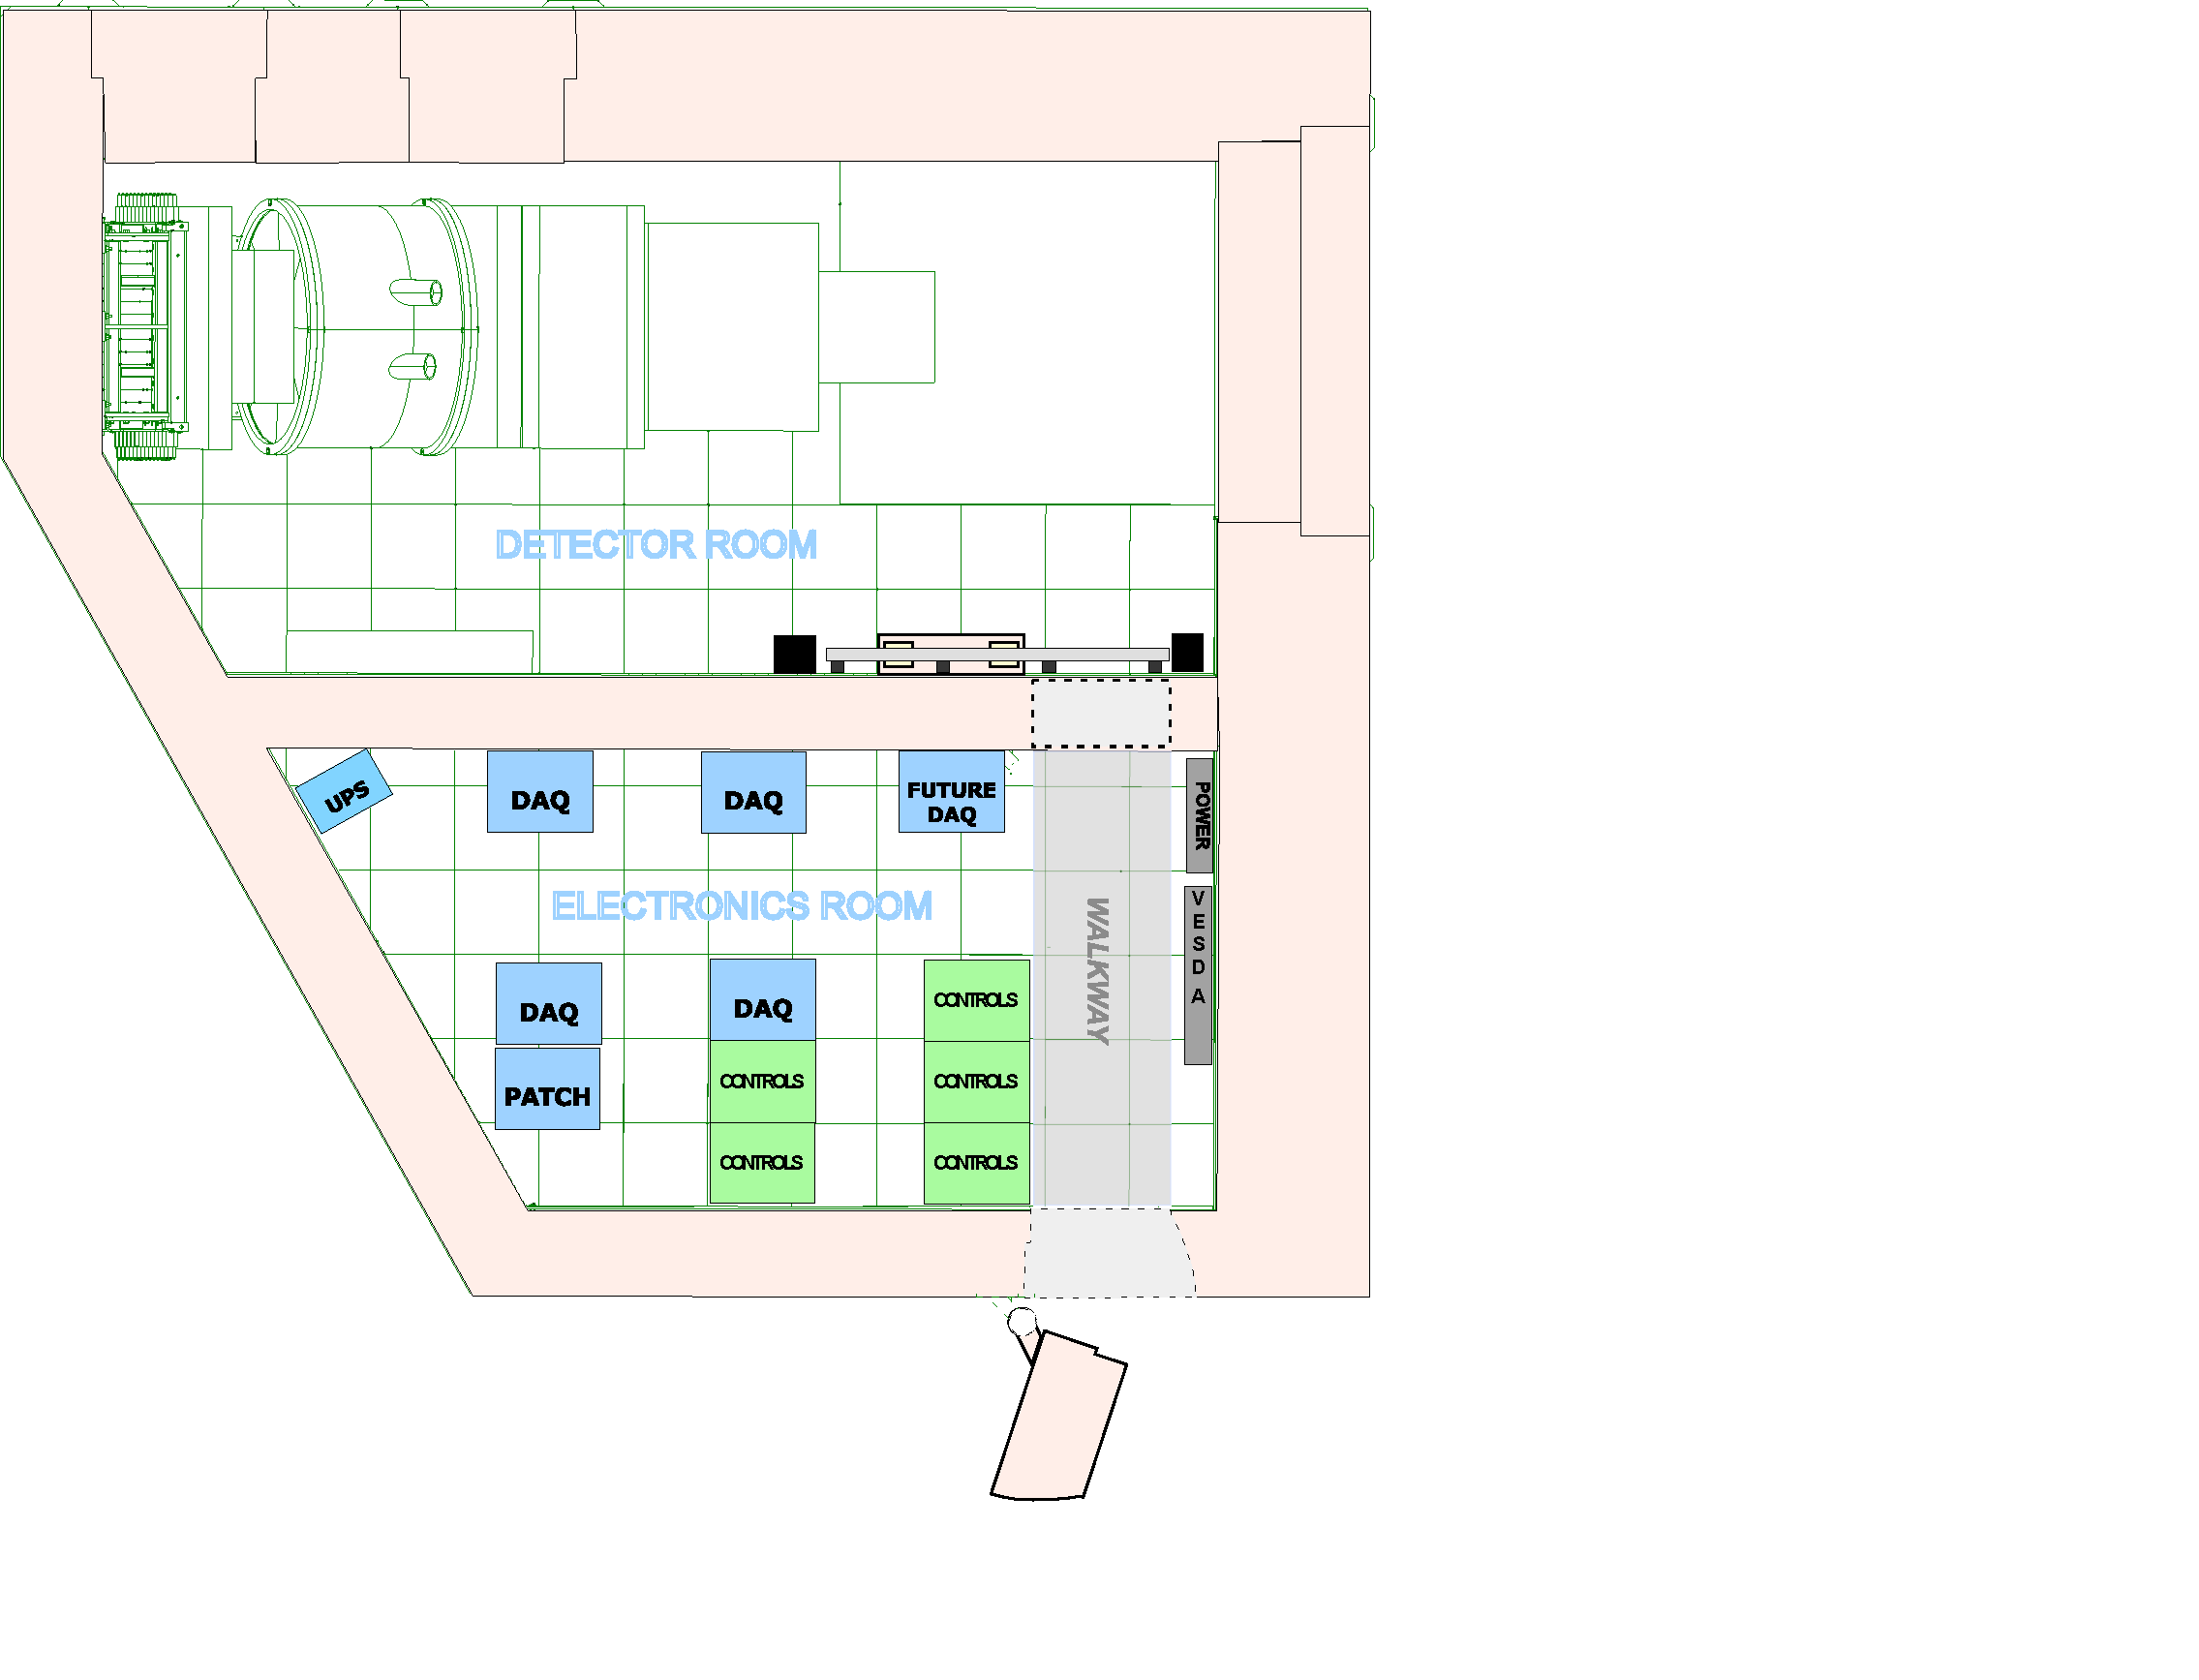
\includegraphics[width=5in]{ShieldHutRacks_hcfAsBuilt.pdf}
\caption{\label{fig:shmshuts}SHMS Detector and Electronics huts,
  accessible from the second level of the SHMS structure.  The
  detectors are accessible by passing through the electronics room.}
\end{center}
\end{figure}

\begin{figure}
\begin{center}
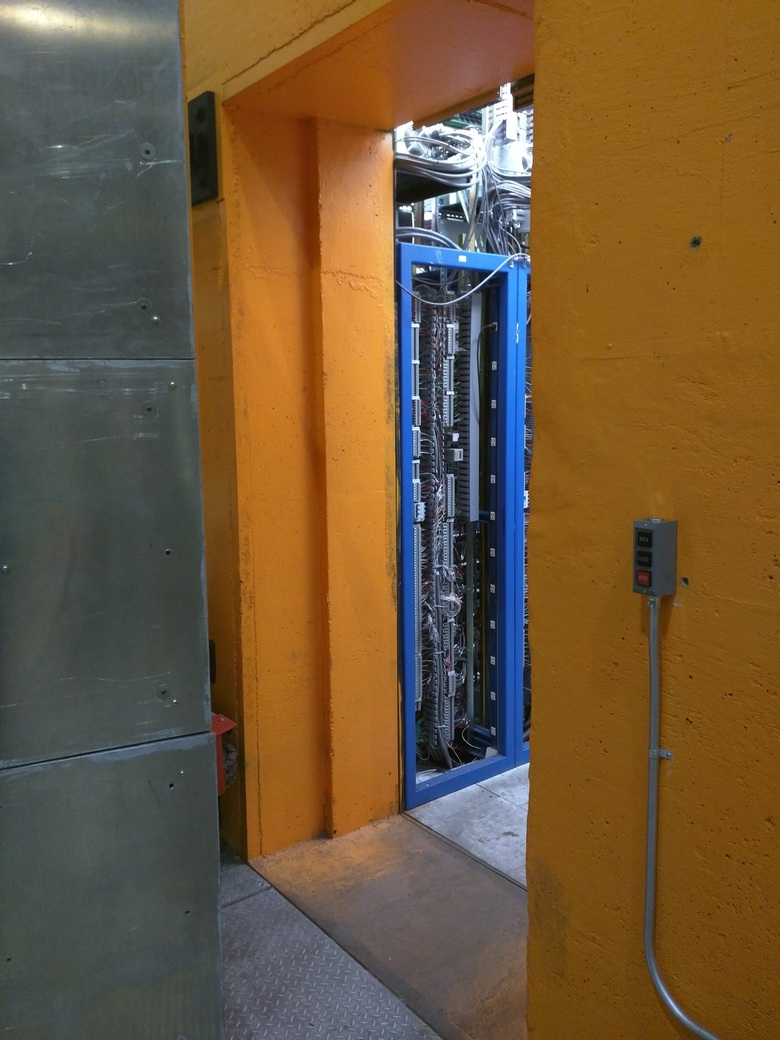
\includegraphics[width=4in]{shmsdoor.jpg}
\caption{\label{fig:shmsdoorcontrol}SHMS hut outside door control buttons.}
\end{center}
\end{figure}

\subsection{SHMS Electronics and Detector Shield Hut Doors}
\label{sec:shmsdoors}
The SHMS electronics shield hut is accessed through concrete door held
closed by a magnetic lock.  To open this door, press and hold the
button marked OPEN.  (Figure~\ref{fig:shmsdoorcontrol})  This will
deenergize the magnetic lock and rotate
the door.  When the door is open sufficient for access, release the
button.  To close the door, make sure the door is clear of
obstructions and hold the CLOSE button until the door closes and the
magnetic lock activates.  A duplicate set of controls is located on
the inside of this door.  When the door motor is energized, audible and visual
alarms will be activated.

The detector shield hut is accessed by passing through the electronics
hut and passing through a second door.  This door is a sliding door
(``barn door'') and is operated by the lower set of buttons to the
right of that door (Figure~\ref{fig:barndoorcontrol}).  This door is activated
in the same manner as the outer electronics hut door: The door slides open
while the OPEN button is depressed, slides closed when the CLOSE button
is depressed and movement stops when the button is released.  Audible and
visual alarms are also installed for the sliding door.
If the spectrometer
vaccum window has a shutter installed, then this door may only be
opened if that shutter is closed.  This shutter is described in the
next section.

An emergency bypass is available allowing override of the shutter
interlock on the door.  Hearing protection must be worn if detector
hut is accessed while the shutter is open and the spectrometer is
under vacuum.

\begin{figure}
\begin{center}
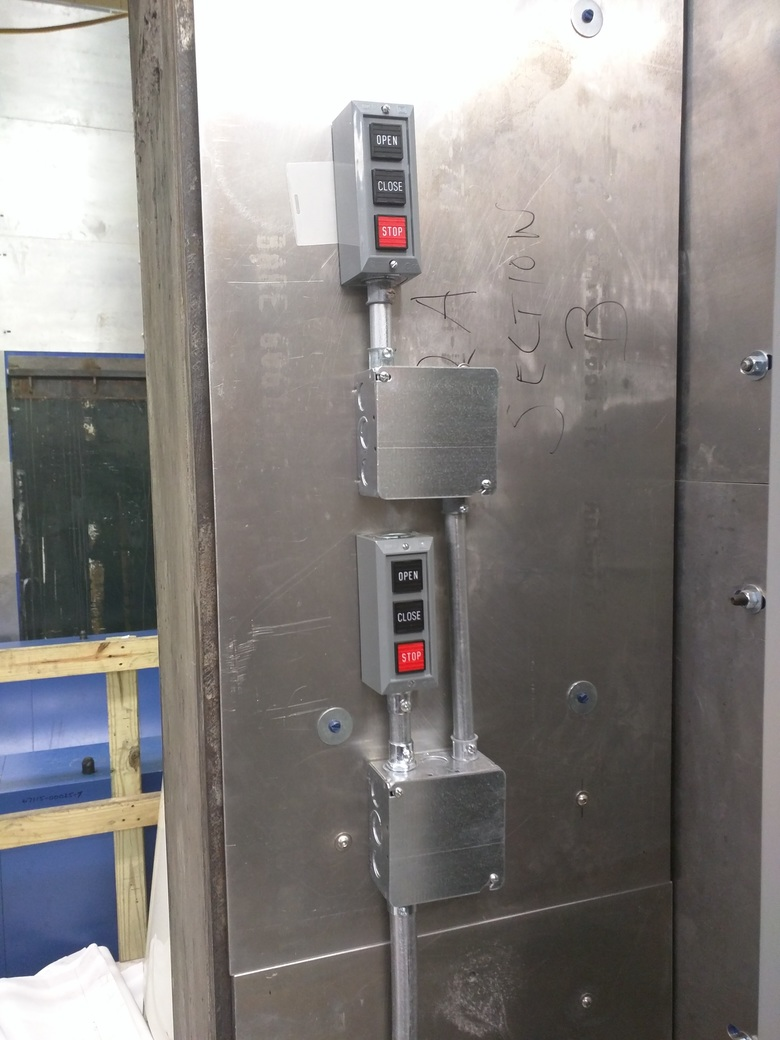
\includegraphics[width=3in]{barndoor-outside.jpg}
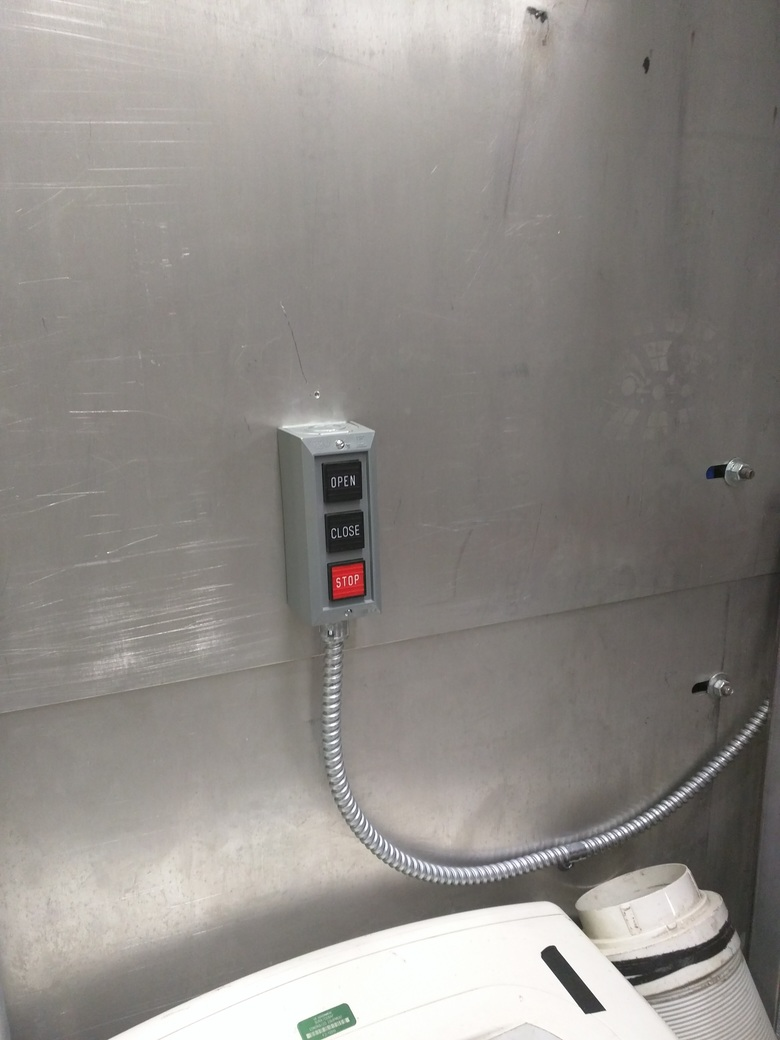
\includegraphics[width=3in]{barndoor-inside.jpg}
\caption{\label{fig:barndoorcontrol}SHMS barn door controls.  The left
  picture shows the controls located in electronics hut.  The bottom
  buttons control the barn door. The top buttons control the SHMS
  vacuum extension shutter.  Below the shutter controls are lights
  indicating if the shutter is opened or closed.  The right picture
  shows the barn door controls located inside the detector hut.}
\end{center}
\end{figure}

\subsection{SHMS Vacuum Window Shutter}
\label{sec:shmsshutter}
As described in section~\ref{sec:shmswindows}, there is a large thin
vacuum window at the end of the vacuum pipe in the SHMS detector hut.
Because of
the considerable stored energy in such a large vacuum volume, it is
necessary to protect the window from accidental puncture by
tools and equipment.
If
the Noble Gas Cherenkov detector is installed, protection is provided
by that detector.
If the Noble Gas Cherenkov is not installed, a vacuum
extension pipe, with a window further into the detector hut will be
used.  In this case, the window will be covered by a shutter to
protect the window from being punctured by tools.
This shutter must be in place whenever the spectrometer is under vacuum and
the ``barn door'' is open.  The shutter is operated by using the top
set of buttons shown in Fig.~\ref{fig:barndoorcontrol}.  To open or close
the shutter, momentarily press the OPEN or CLOSE button.  The shutter will move
until it reaches the open or closed state. (Unlike the door controls,
the button does not need to be held down.)  Indicator
lights near the shutter and door controls show whether the shutter is open or closed.




}%\infolevone
